\documentclass{article}[12pt]
\usepackage{graphicx}
\usepackage{amsmath}
\usepackage{indentfirst}
\usepackage{color}
\usepackage{cite}
\usepackage{wasysym}
\usepackage{amssymb}
\usepackage{multirow}
\usepackage{subcaption}
\usepackage{float}



% --Defining Parameters--
\oddsidemargin -0.25in		% Left margin is 1in + this value
\textwidth 6.75in		% Right margin is not set explicitly
\topmargin -0.25in		% Top margin is 1in + this value
\textheight 9in			% Bottom margin is not set explicitly
\columnsep 0.25in		% separation between columns

% -- Change Section Numbers for Roman Numerals -- 
\renewcommand{\thesection}{\Roman{section}} 
\renewcommand{\thesubsection}{\thesection.\Roman{subsection}}
\renewcommand{\figurename}{Fig. }
\renewcommand\refname{REFERENCES}






\begin{document}

\title{Optical Spectra}
\author{Samuel Barton}


%--- Heading ---
\begin{center}
\large{\textbf{Optical Spectra}}\\
\bigskip
\small{Samuel Barton}\\
\small{\textit{Department of Physics \& Astronomy, Dartmouth College, Wilder Laboratory, Hanover, NH, USA}}\\
~\\
\small{\textbf{Partner:} Alex Ward; \textbf{Lab Section:} Thursday }\\
~\\
Dated: October 30, 2023\\

\end{center}

%--- Abstract ---
\bigskip
\begin{abstract}
  This lab had three primary objectives.
  The first was to observe how much the background noise measured by the sensor follows a gaussian distribution. Furthermore, we learned how to manipulate the software - fiddling with detection period and detections to acerage - to reduce noise and provide an ideal tool for data collection, reducing noise.
  The second objective was to look at spectrographs created by different souces of light to determine whether the photons are a result of blackbody radiation, or from electrons changing orbit levels.
  The third and final objective was to determine planck's constant comparing the spectrographs of different LEDs (and their prominent wavelength) to the voltage across them.
  We observed through plotting noisy areas of the spectrograph on a histogram that standard gaussian noise was followed by the light intensity.
  Furthermore, as predicted, the gas discharge bulbs looked like those of spectra found online.
  Finally, planck's constant was measured to $ h = 6.33 \times 10^{-34}  $ which has a percent error of 4.53 \%.
\end{abstract}
\bigskip

%--- Introduction ---
\section{Introduction}

In this lab, we worked with the optical spectra of visible (and infrared) light.
The optical spectra for visible light ranges from 380 to 700 nm (see \figurename \ref{vis_light}.

\begin{figure} [H]
  \centering
  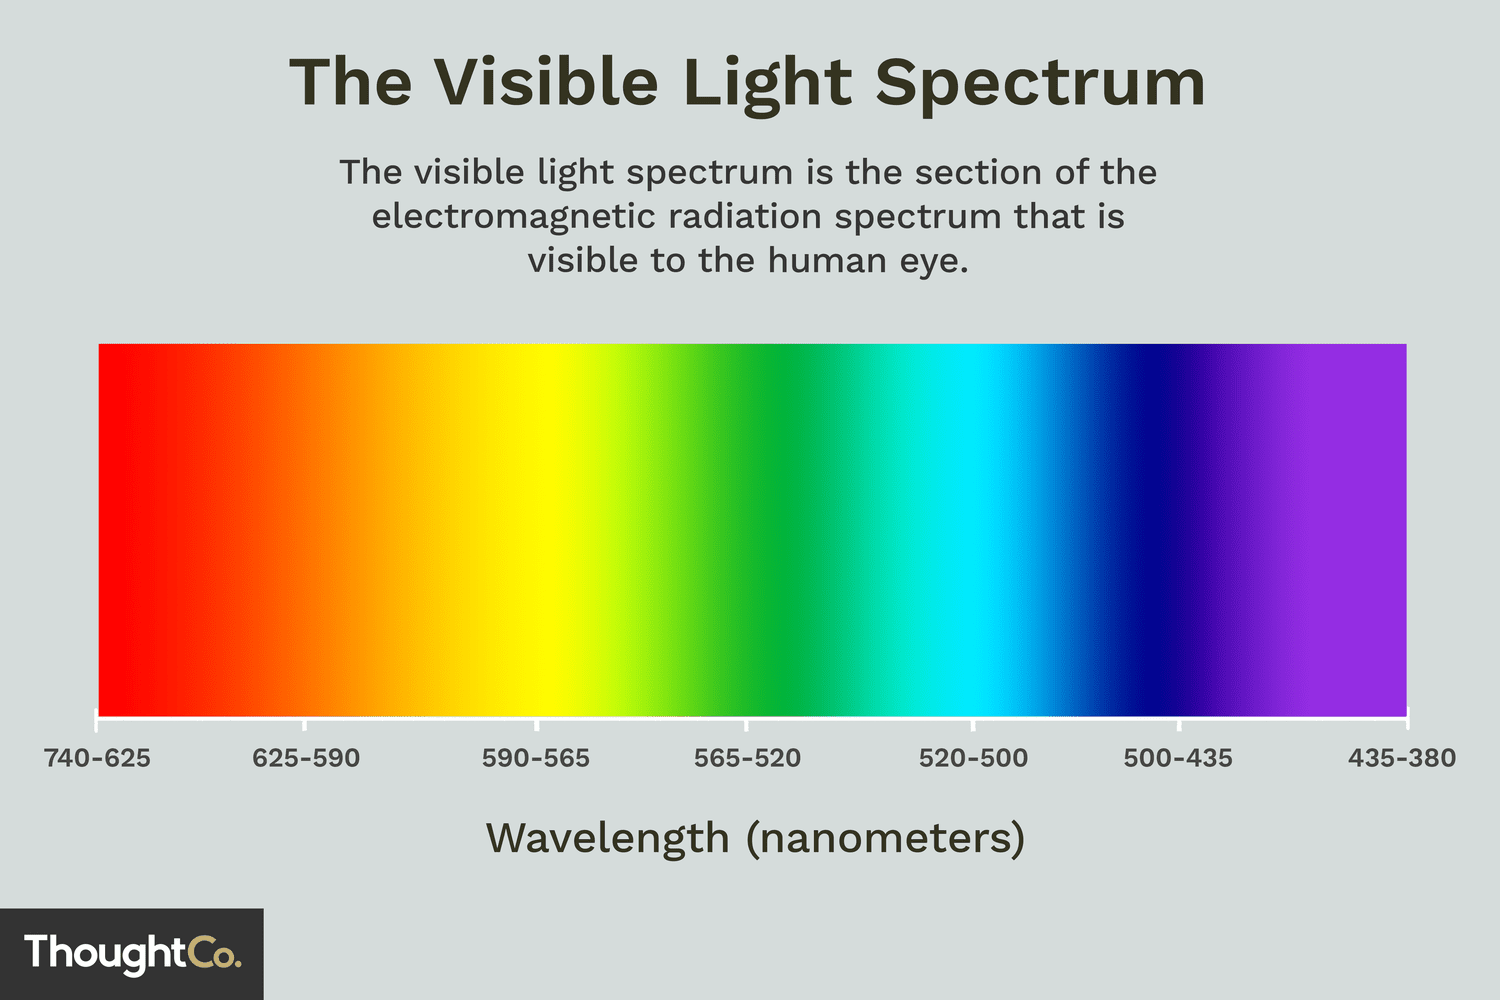
\includegraphics[width=0.45\textwidth]{figures/visible_light_spectrum.png}
  \caption{The Visible Light Spectrum \tiny (from https://www.thoughtco.com/the-visible-light-spectrum-2699036)}
  \label{vis_light}
\end{figure}

In the measurement setup, the light travelled through an fiber-optic tube,and into the spectrometer.
Inside the spectrometer, mirrors reflect photons to a diffraction grating, splitting the protons by wavelength.
The diffraction grating then spreads light across a focusing mirror which directs light at each wavelength onto the detector.
At the detector, light strikes the CCD (Charge Coupled Device) at different pixels, and each pixel represents a portion of the spectrum which is then translated into an answer with spectroscopy software.
In our lab, this spectroscopy software and hardware was OceanView, and it measured wavelengths ranging from 200 to 900 nm, greater than the spectrum of visible light.
The OceanGate software also has a few important functions for data visualation and calculation:
The integration time parameter varies the duration of time that the software collects data before creating the graph.
A longer duration correlates with more photons being collected, and a graph with higher intensities.
The number of averages parameter changes the number of datasets the program collects before averaging the datapoints and displaying the averages as a graph.
A higher number of averages reduces the background noise, but requires more cycles of data collection to display a graph.

Light sources can be differentiated by the mechanism for which they emit electromagnetic (EM) radiation.
Some light sources emit a large range of EM radiation through blackbody radiation.
Other light sources emit photons as a result of electrons falling to a lower energy orbital state, resulting in a set wavelength characteristic to the specific atom itself. 

Another important concept in this lab was that of statistical noise, and Gaussian/Normal distribution more specifically. 
When using the optical spectrometer, variations in the intensity of light, as well as the number of electrons striking the CCD lead to random fluctuations in the measured intensity.
This probability distribution most commonly represents the Gaussian or Normal distribution where:

\begin{equation}
  P(x) = \frac{1}{\sqrt{2 \pi \sigma ^2}} e ^{-\frac{(x-\mu )^2}{2 \sigma ^2}} 
\end{equation}
Where $ \sigma   $ is the standard deviation and $ \mu  $ is the mean.

We expect that in relatively flat (and noisy) regions in wavelength, the intensity will follow this Gaussian Distribution.
Finally, we return again to the concept of planck's constant in this lab.
Planck's constant:
\begin{equation}
  h = 6.626 \times 10 ^{-34}~\mathrm{J\cdot s}
\end{equation} 

Furthermore, we have the equation:

\begin{equation}
  E=hf
  \label{ehf}
\end{equation}

%--- Method ---
\section{Method}

\noindent \textbf{Equipment:}

In \figurename \ref{spectrometer} you can see an illustration of the digital spectrometer from the lab.
In brief, the spectrometer has a narrow internal slit, a transmission grading and a CCD detector fed to via an optical fiber cable.

\begin{figure}
  \centering
  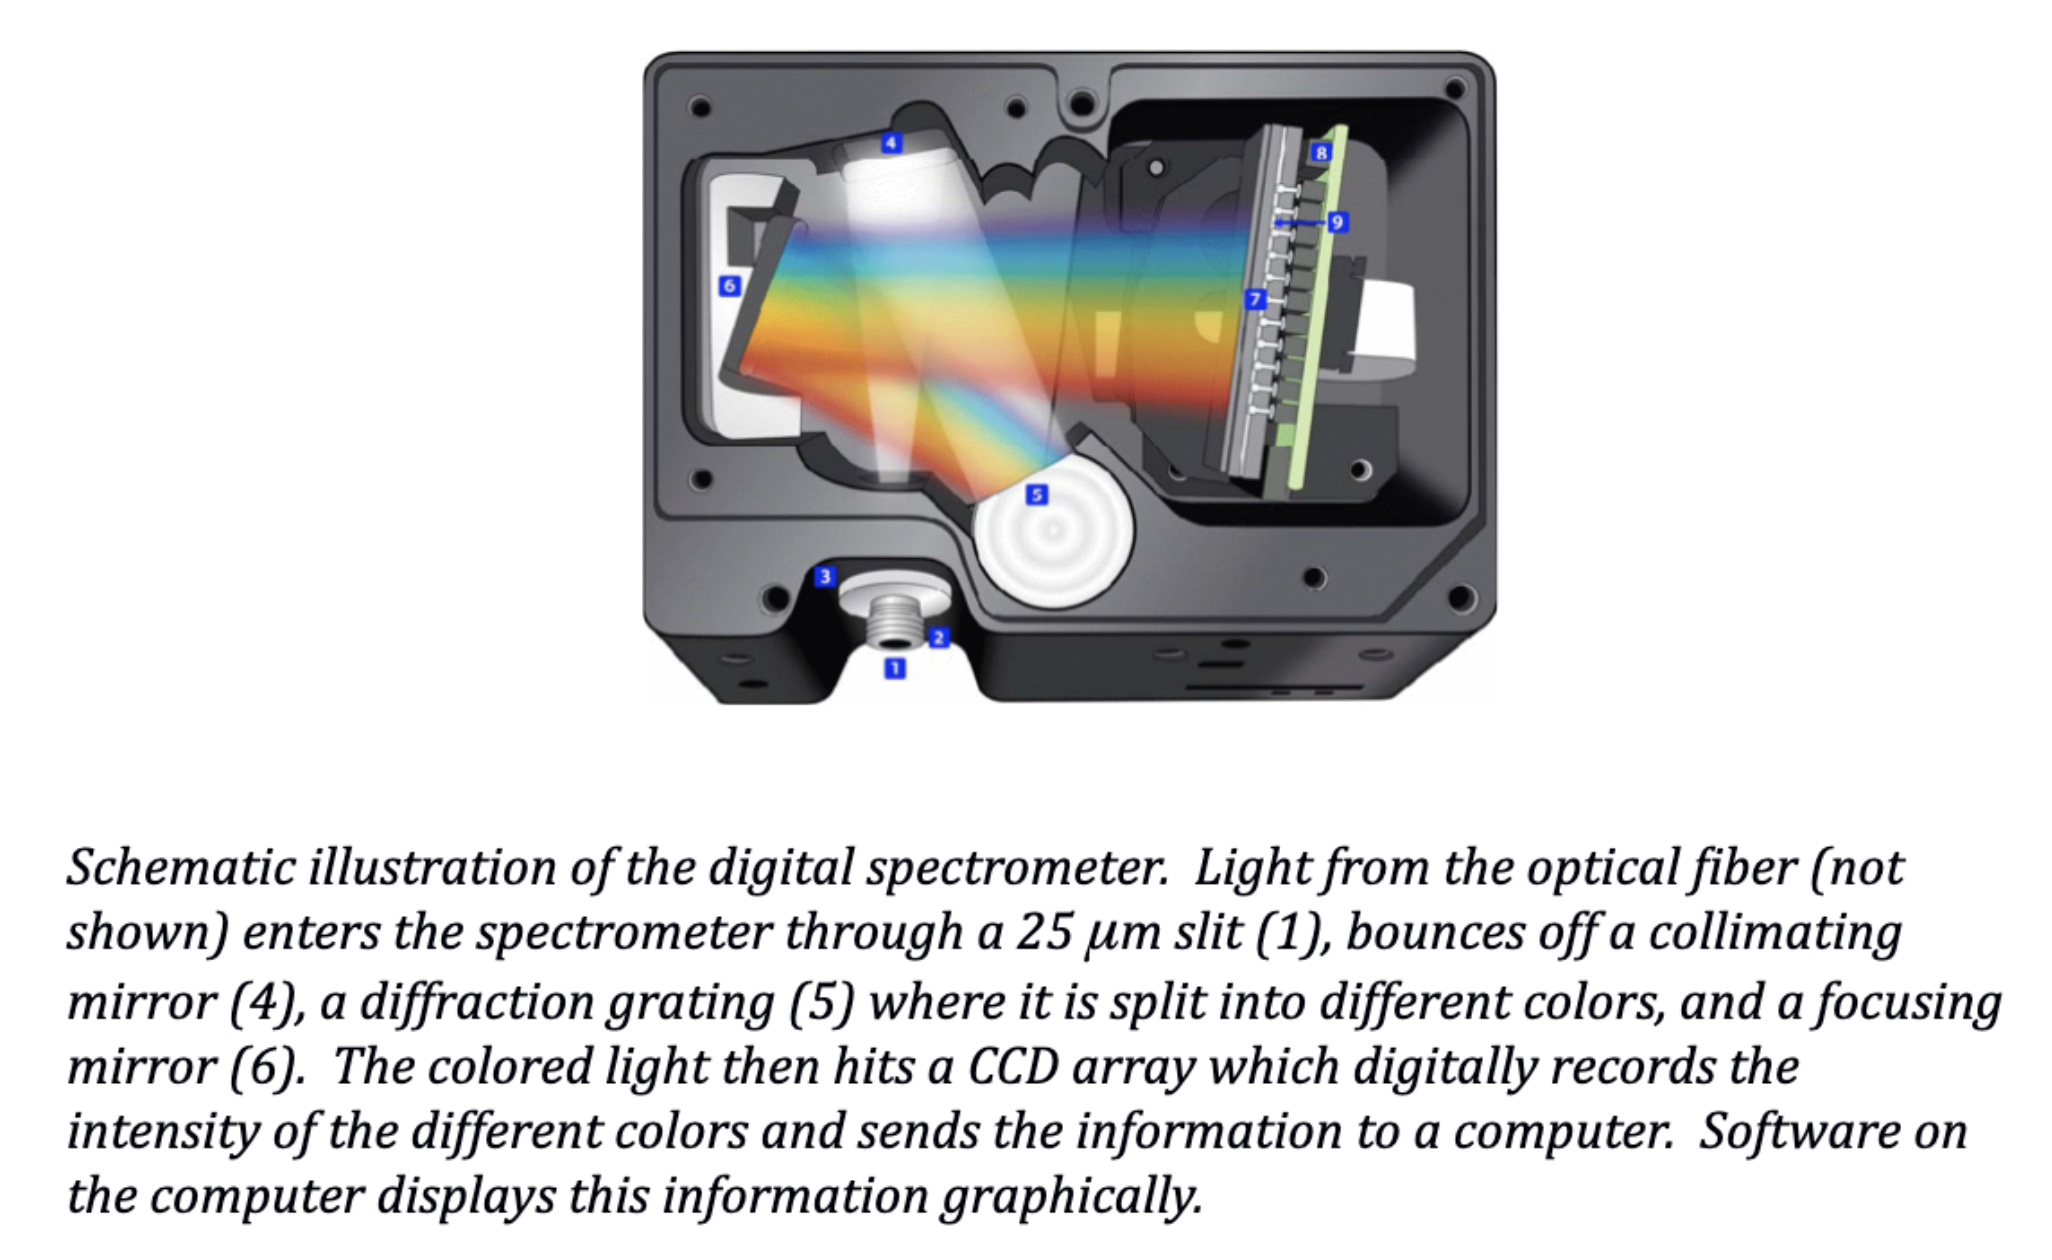
\includegraphics[width=0.65\textwidth]{figures/spectrometer.png}
  \caption{Digital Spectrometer Illustration}
  \label{spectrometer}
\end{figure}

\noindent \textbf{Procedure:}

For Investigation 1 we observed a gas-discharge tube, and played around with the integration time and the number for average, before setting them to 100 ms and 5 respectively, saving the dataset.

For Investigation 2 we observed the spectra of many different light sources (2 different gas-discharge tubes, an incandescent bulb, a flourescent buld, a halogen bulb, LED lamp, and 2 lasers with diffusers). We made sure to keep the end of the optical fiber the same distance from the light source for consistency's sake.

For Investigation 3, we connected an LED to a 9-V battery, and measured the voltage across the LED.
We repeated this step with 4 different LEDs, measuring the wavelength (observed from the spectrograph), and the voltage (measured on the multimeter).

\begin{figure}
  \centering
  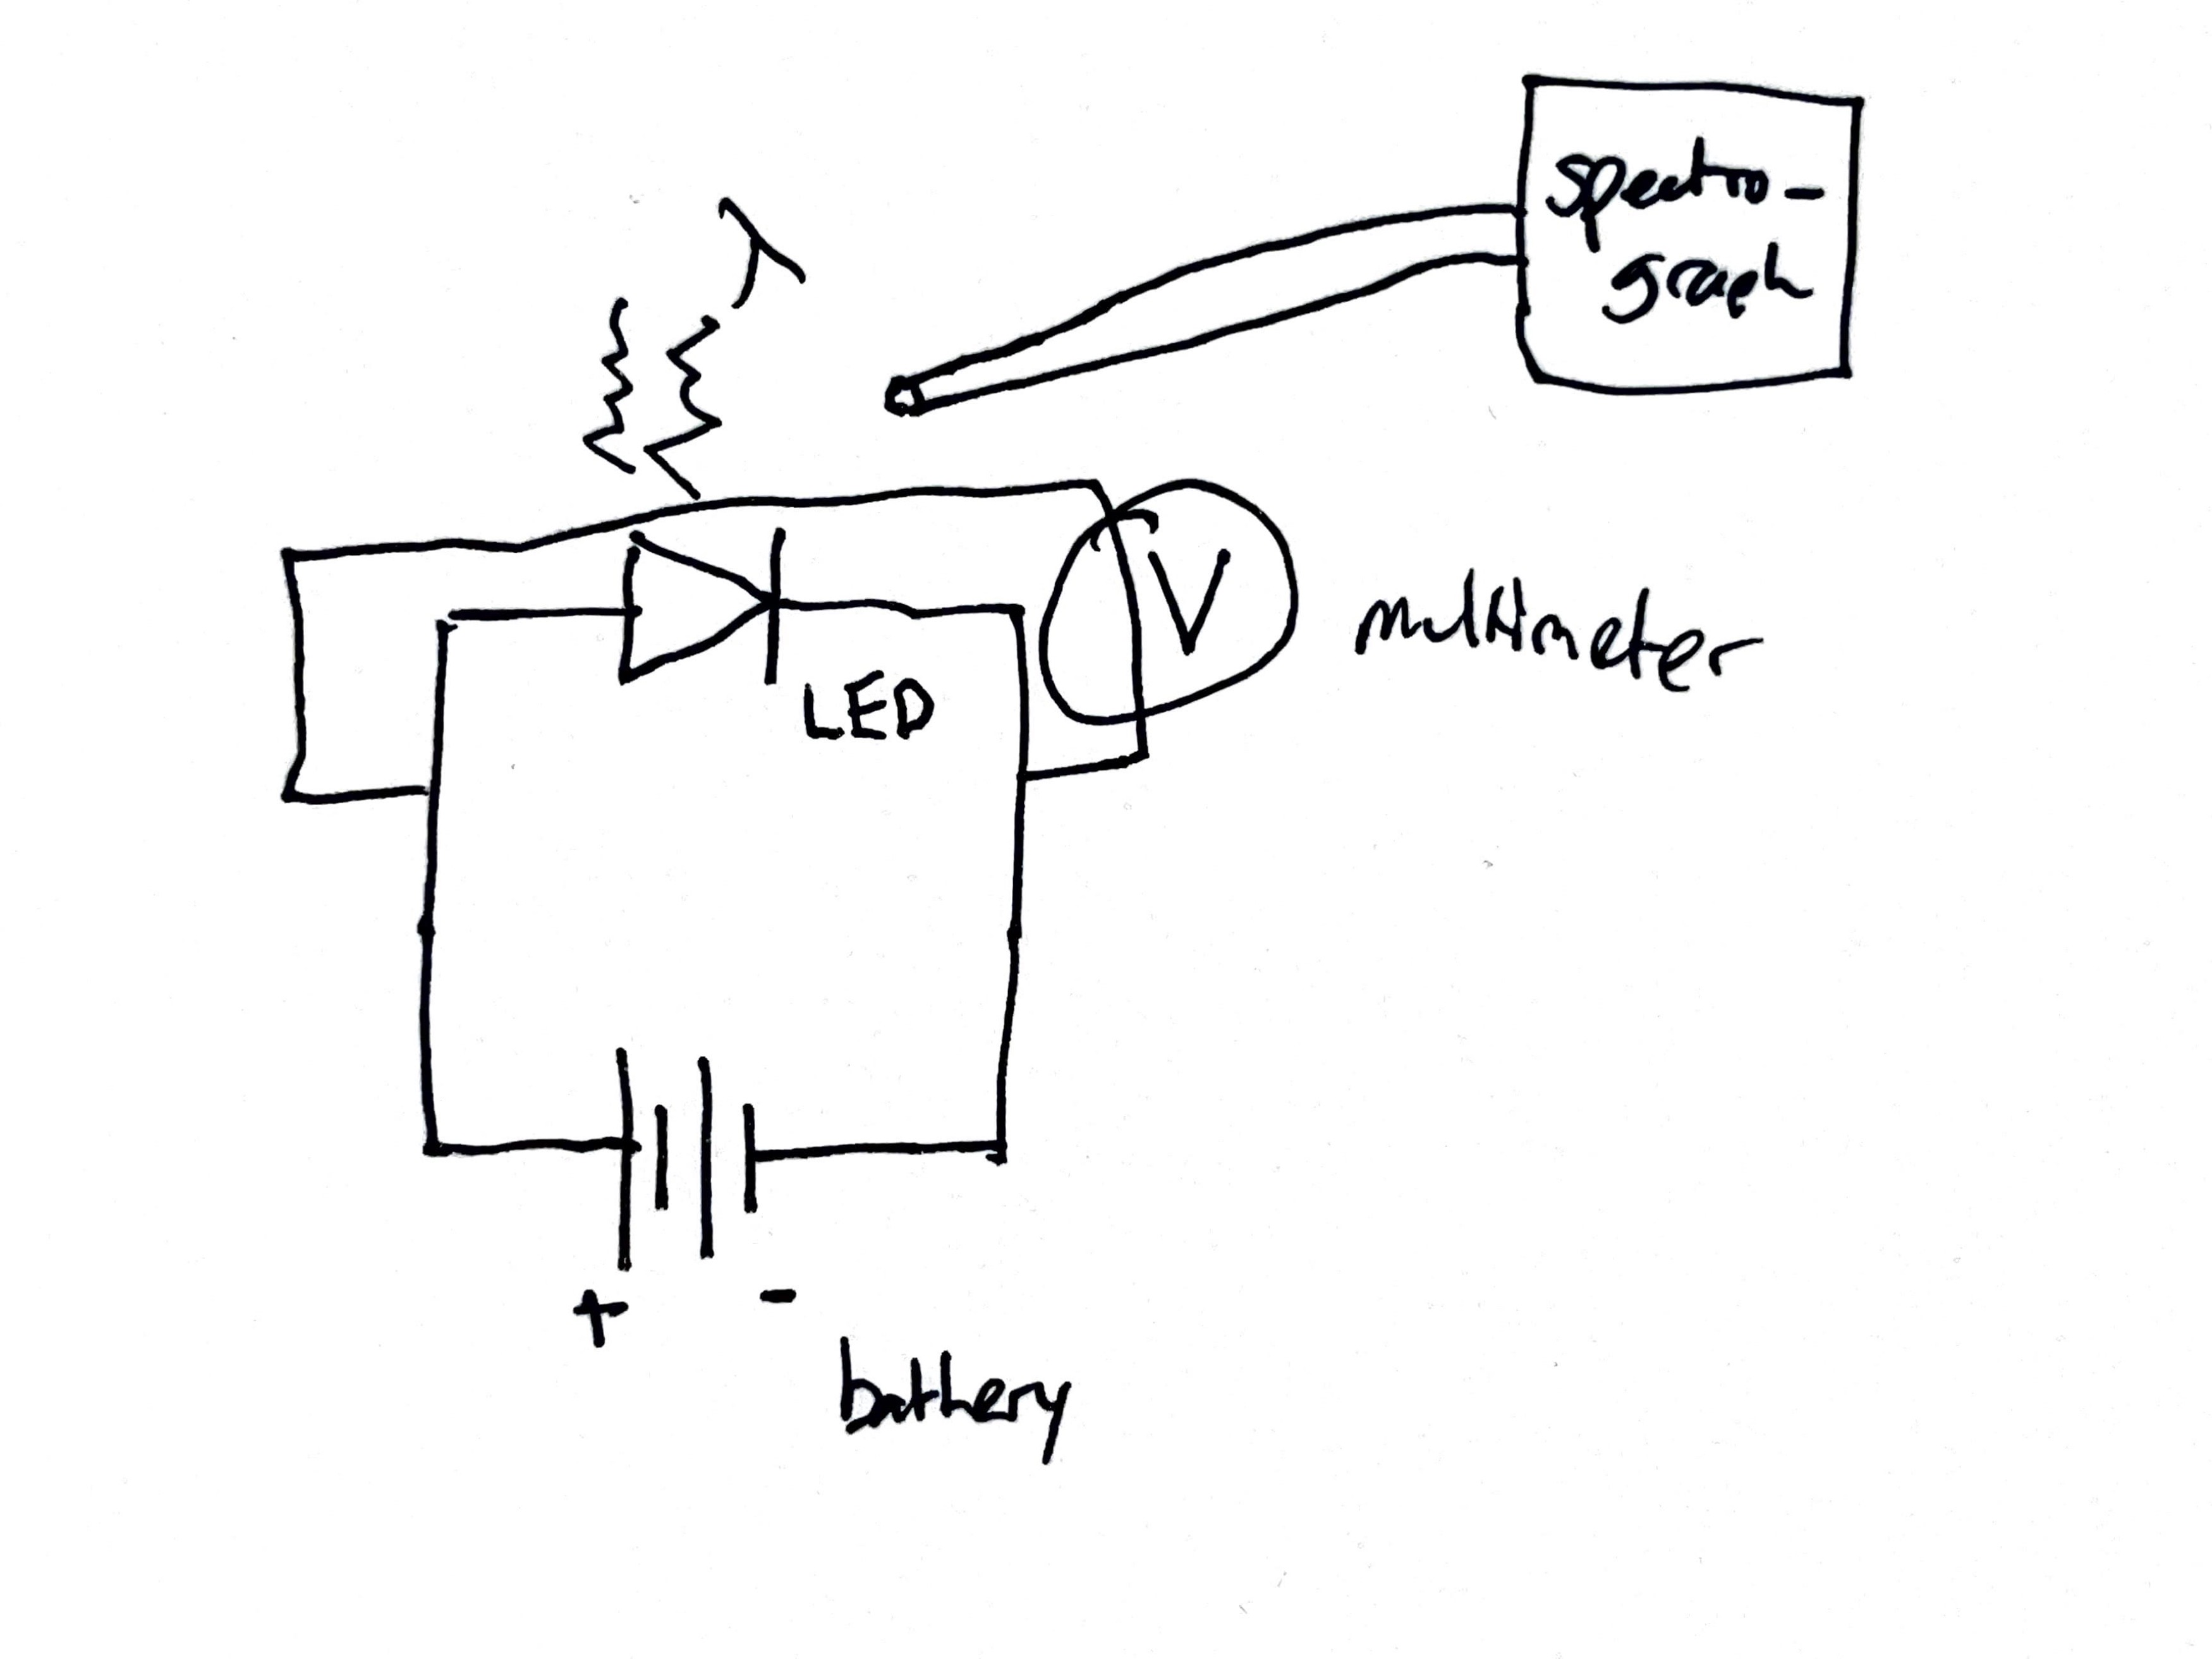
\includegraphics[width=0.65\textwidth]{figures/inv3fig.jpg}
  \caption{Diagram of Investigation 3 Setup}
\end{figure}


%--- Data ---
\section{Data}

\subsection{Investigation 1}

\begin{figure} [H]
  \centering
  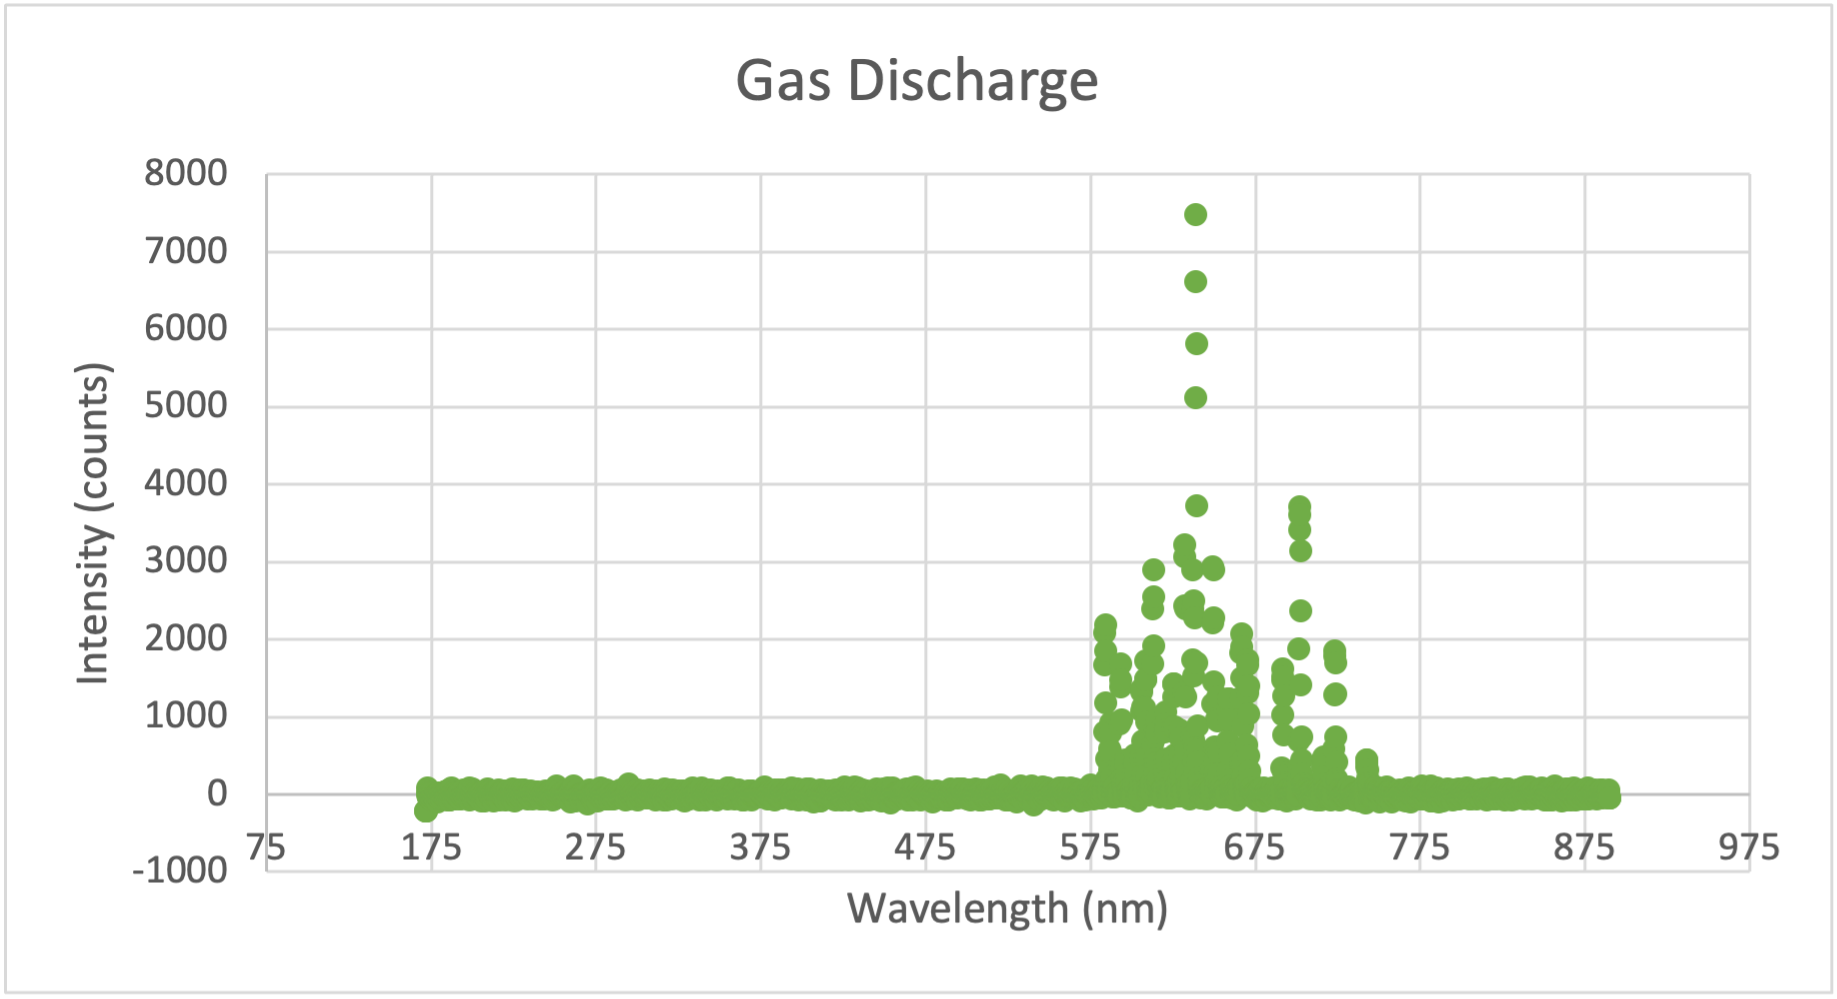
\includegraphics[width=0.65\textwidth]{figures/gas1spec.png}
  \caption{Gas Discharge Tube 1 Spectrograph Data}
  \label{gas1spec}
\end{figure}

\begin{figure} [H]
  \centering
  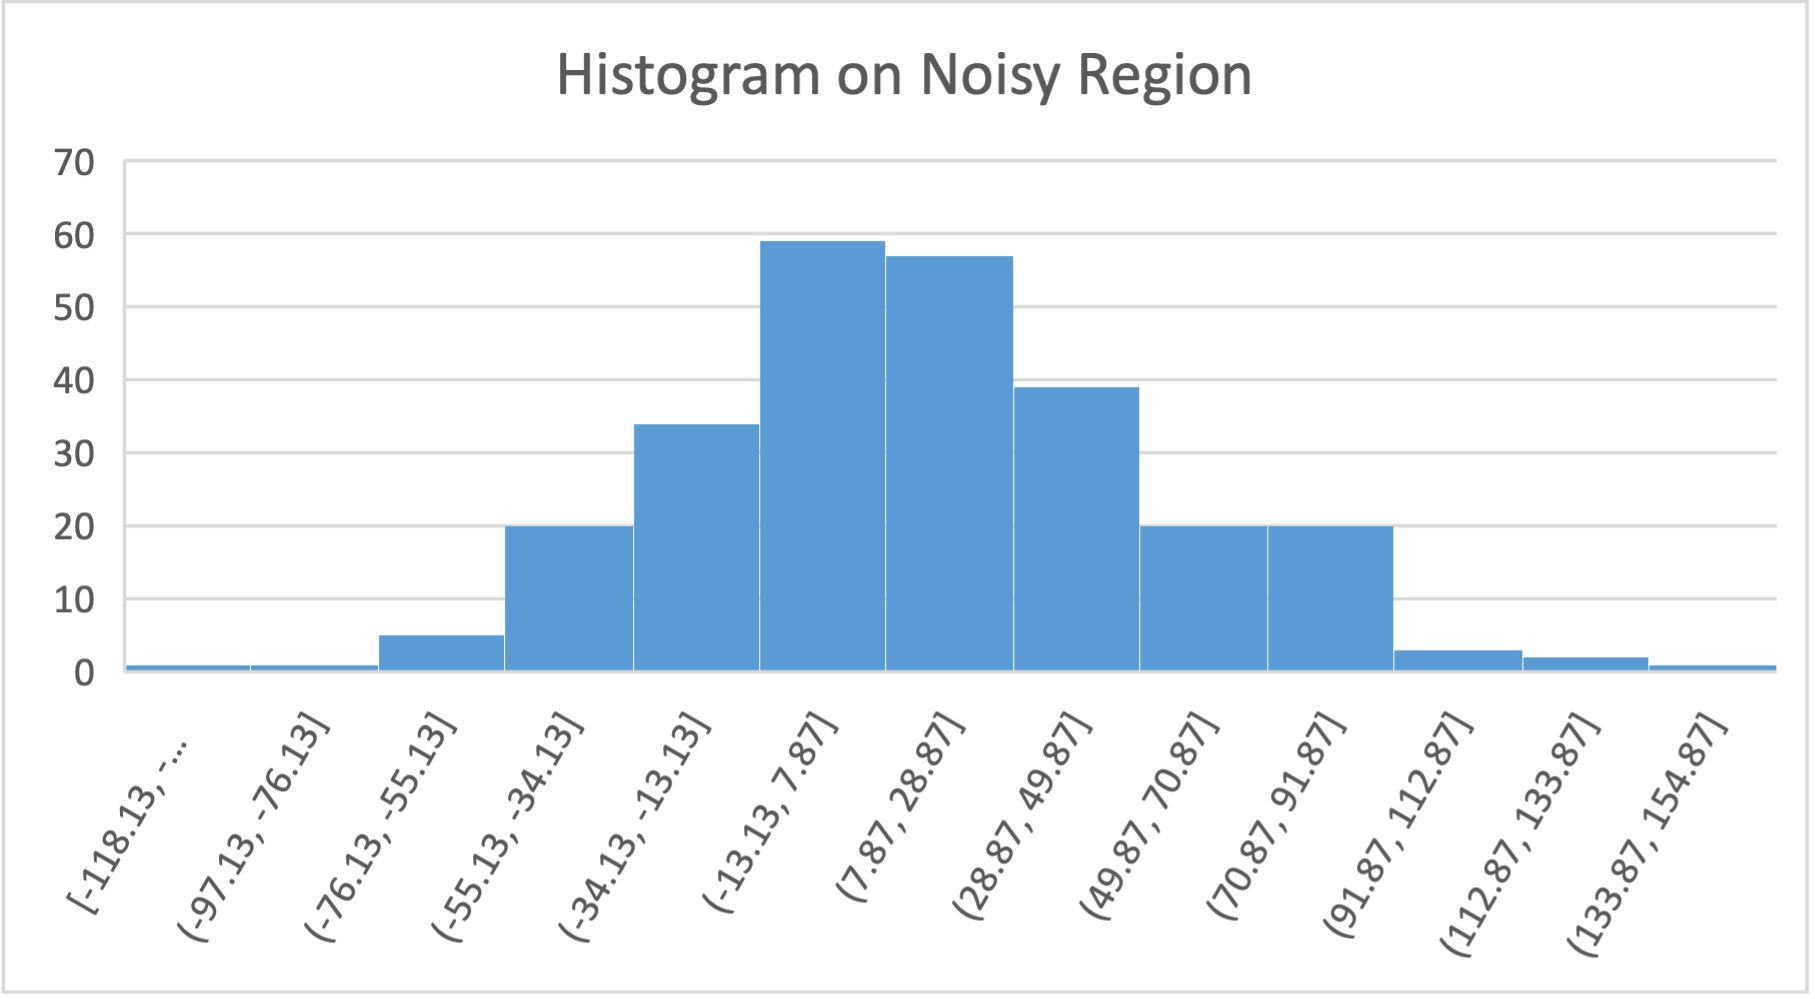
\includegraphics[width=0.65\textwidth]{figures/histo.png}
  \caption{Histogram on a 50 nm Flat \& Noisy Region of Gas Discharge Tube spectrograph}
  \label{histo}
\end{figure}

\subsection{Investigation 2}

For Investigation 2, we captured screenshots of various spectra from different light sources.

\begin{figure} [H]
  \centering
  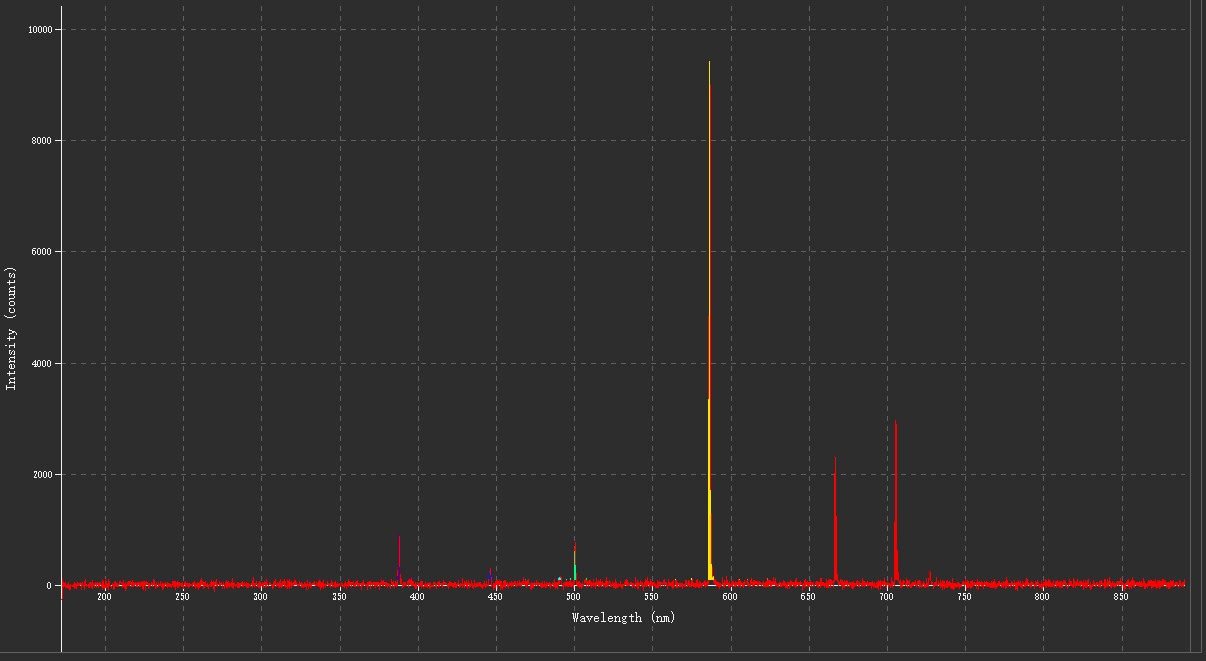
\includegraphics[width=0.65\textwidth]{figures/gas2.png}
  \caption{Spectrograph for Gas Discharge 2 (note the distinct intensity peaks, indicating that they ar formed by discrete energy levels)}
  \label{gas2}
\end{figure}

\begin{figure} [H]
  \centering
  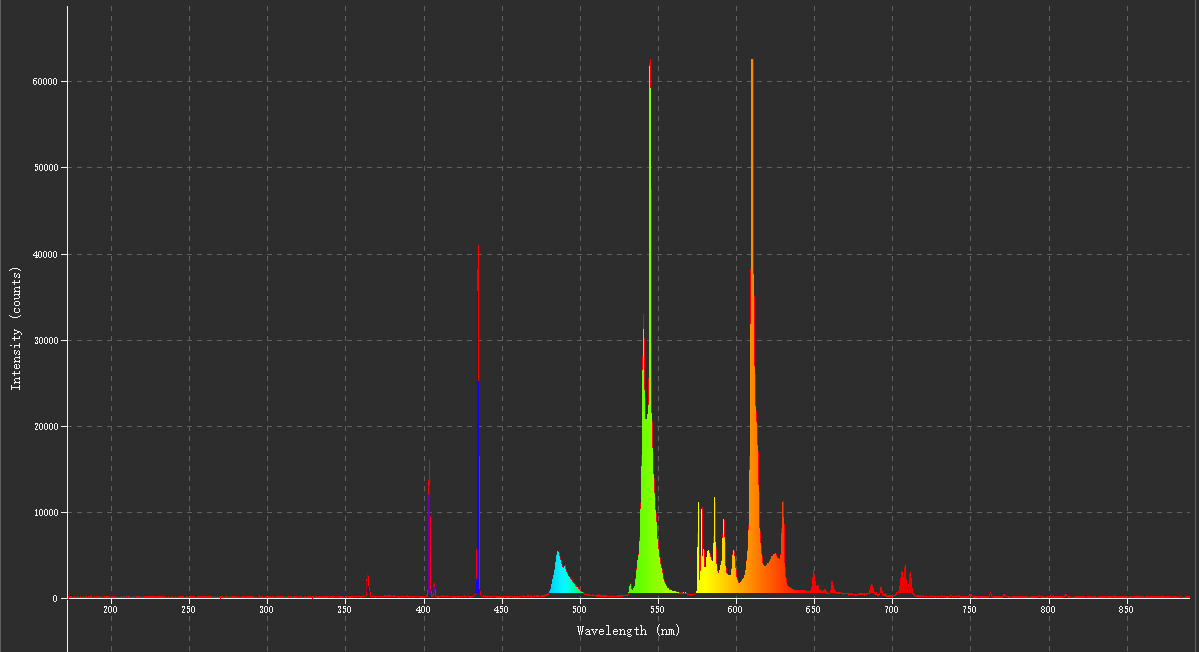
\includegraphics[width=0.65\textwidth]{figures/flourescent.png}
  \caption{Spectrograph for the Flourescent Bulb}
  \label{flour}
\end{figure}

\begin{figure} [H]
  \centering
  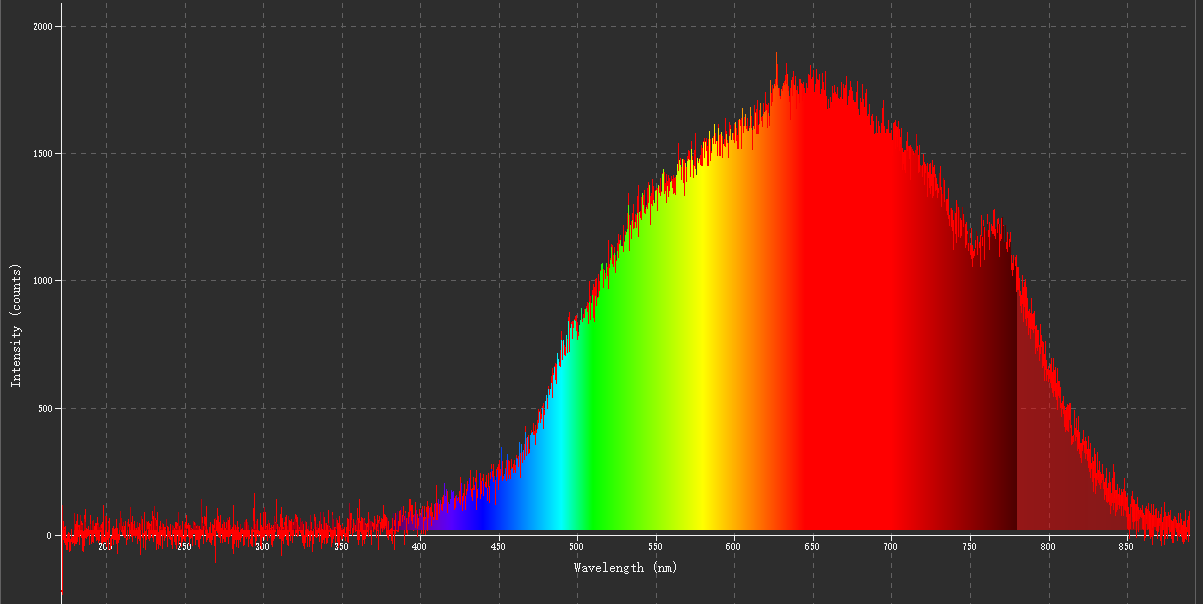
\includegraphics[width=0.65\textwidth]{figures/incandescent.png}
  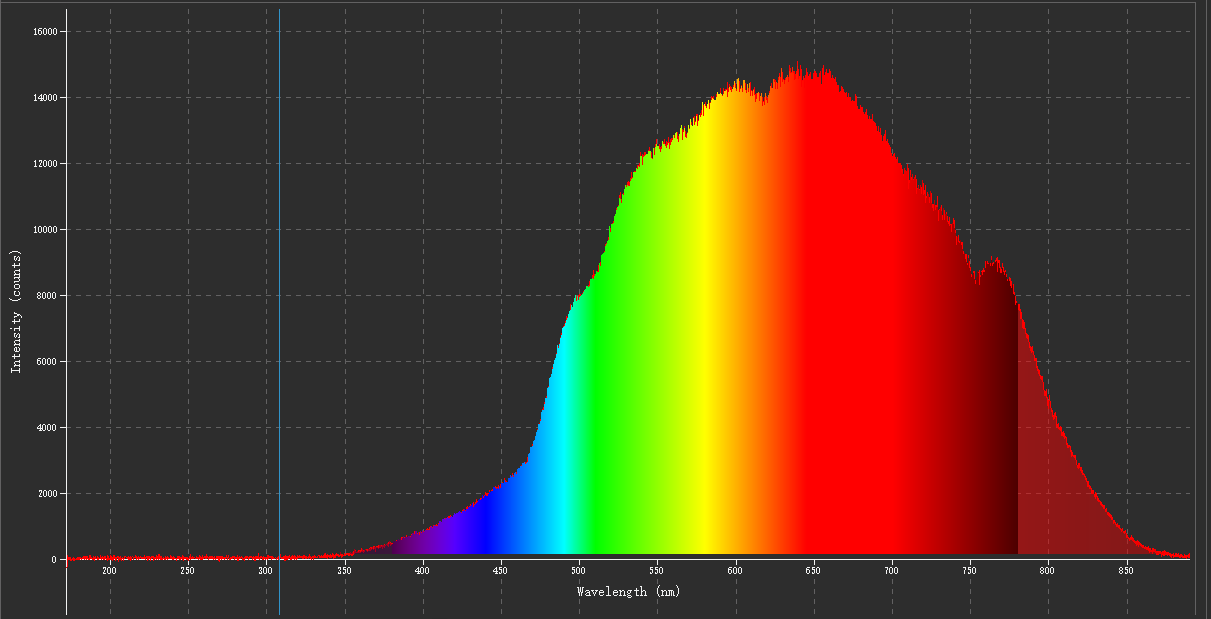
\includegraphics[width=0.65\textwidth]{figures/halogen.png}
  \caption{Spectrographs for the Incandescent and Halogen Bulbs}
  \label{bbrad}
\end{figure}

\begin{figure} [H]
  \centering
  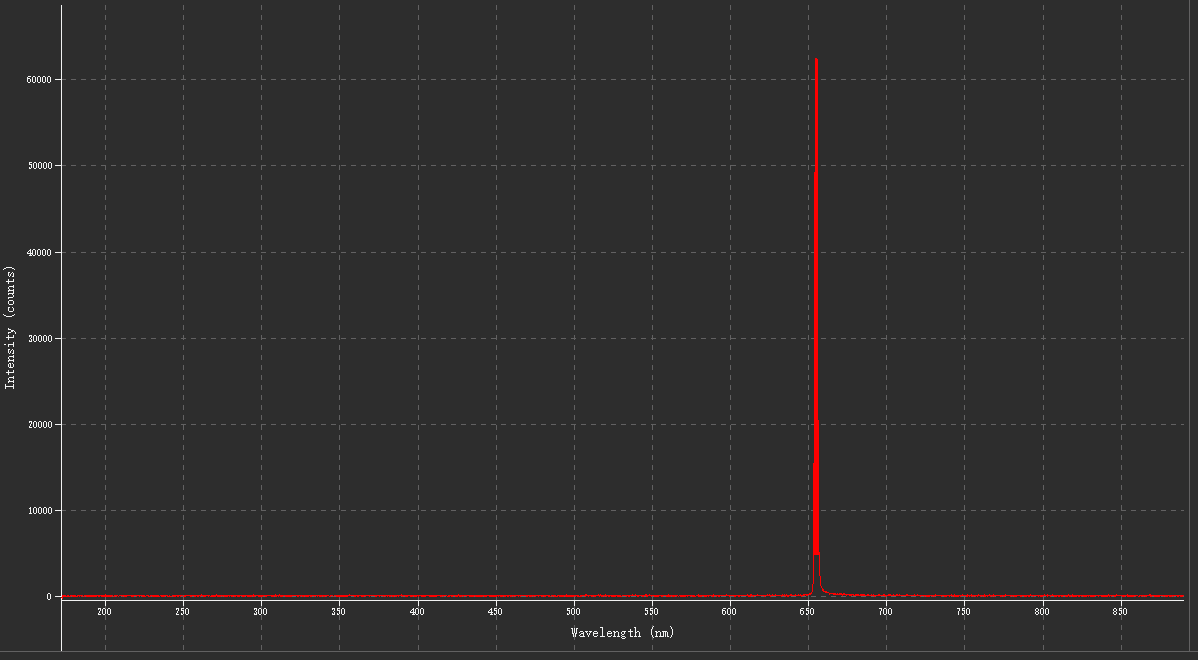
\includegraphics[width=0.65\textwidth]{figures/red_laser.png}
  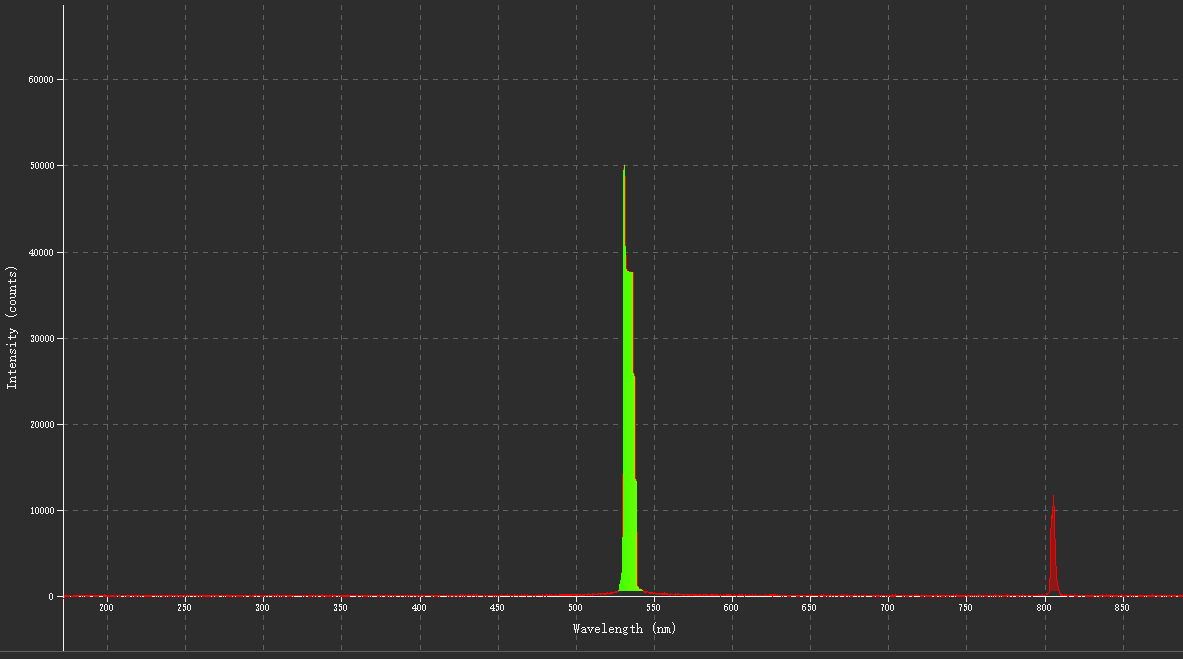
\includegraphics[width=0.65\textwidth]{figures/green_laser.png}
  \caption{Spectographs for Red and Green Lasers}
  \label{lasers}
\end{figure}

\subsection{Investigation 3}

\begin{figure} [H]
  \centering
  \begin{subfigure} [b]{0.475\textwidth}
    \centering
    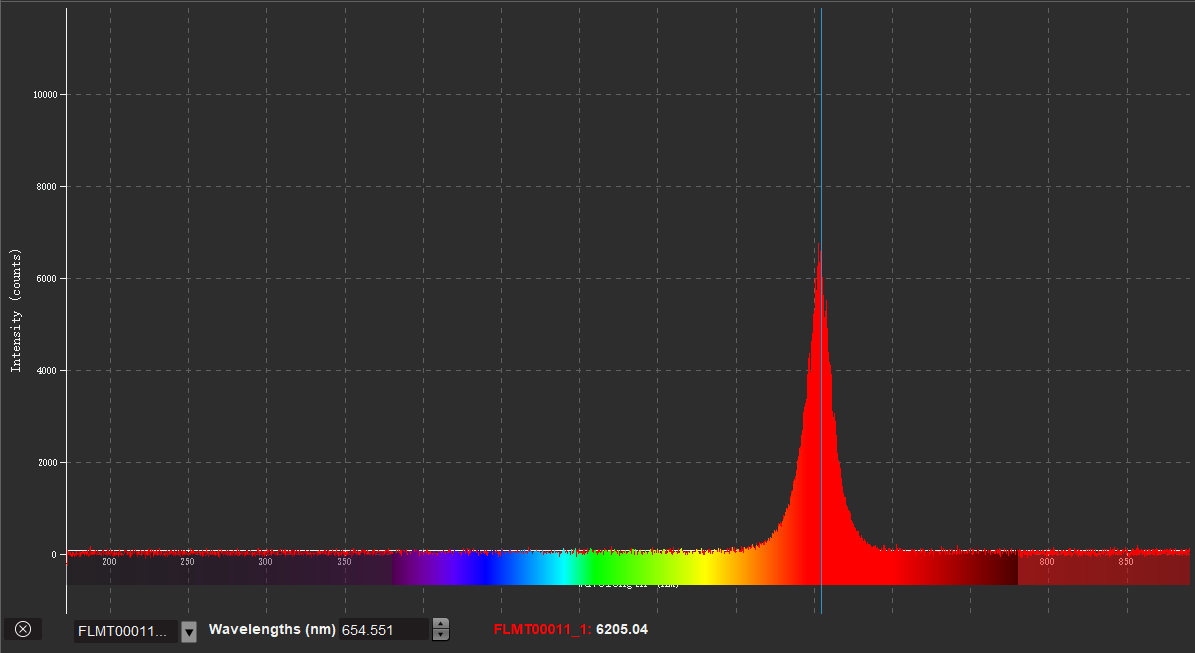
\includegraphics[width=\textwidth]{figures/red_led.PNG}
    \caption{Red LED}
  \end{subfigure}
  \hfill
  \begin{subfigure} [b]{0.475\textwidth}
    \centering
    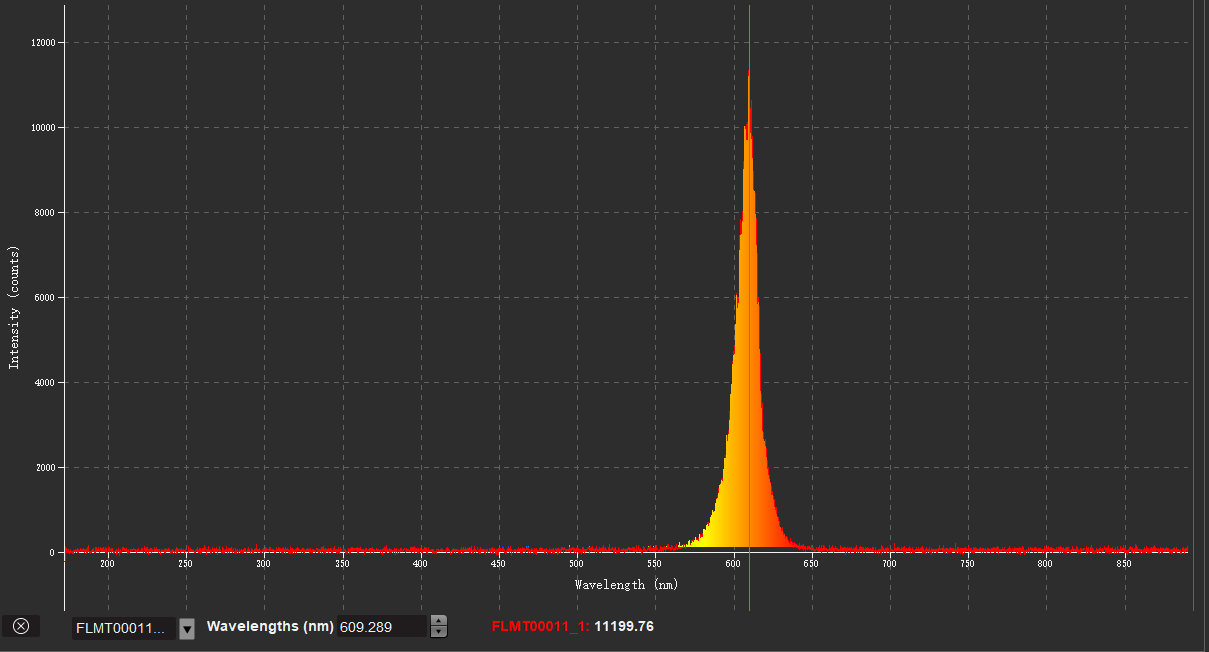
\includegraphics[width=\textwidth]{figures/orange_led.PNG}
    \caption{Orange LED}
  \end{subfigure}
  \vskip\baselineskip
  \begin{subfigure} [b]{0.475\textwidth}
    \centering
    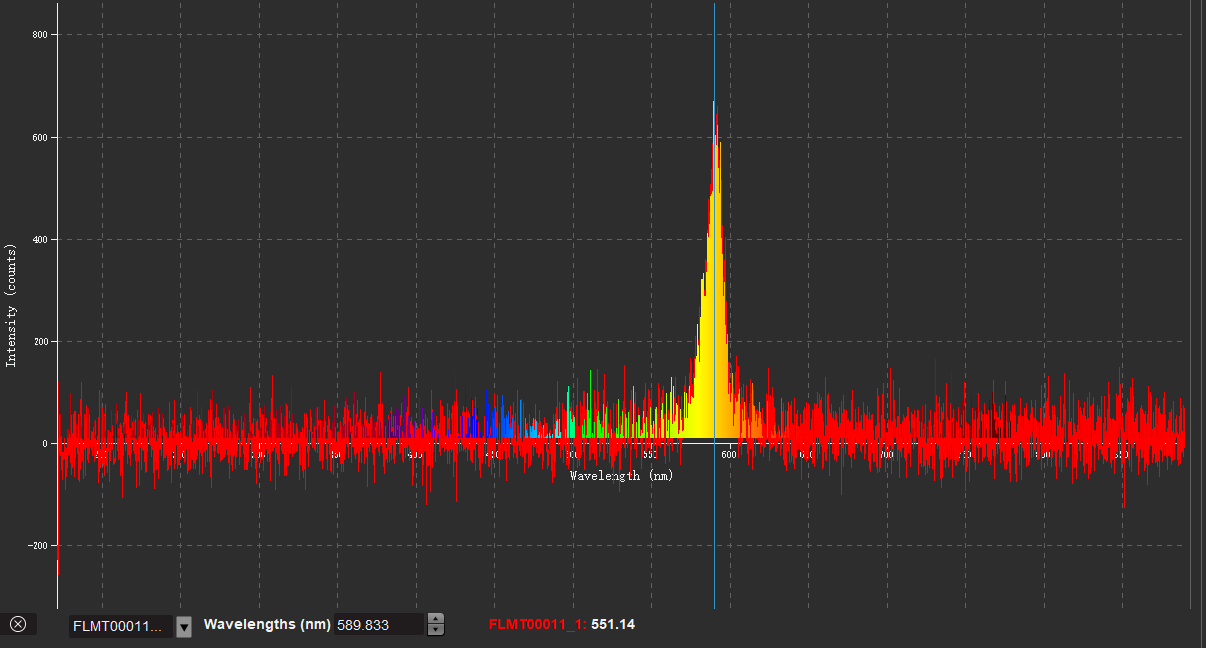
\includegraphics[width=\textwidth]{figures/yellow_led.PNG}
    \caption{Yellow LED}
  \end{subfigure}
  \hfill
  \begin{subfigure} [b]{0.475\textwidth}
    \centering
    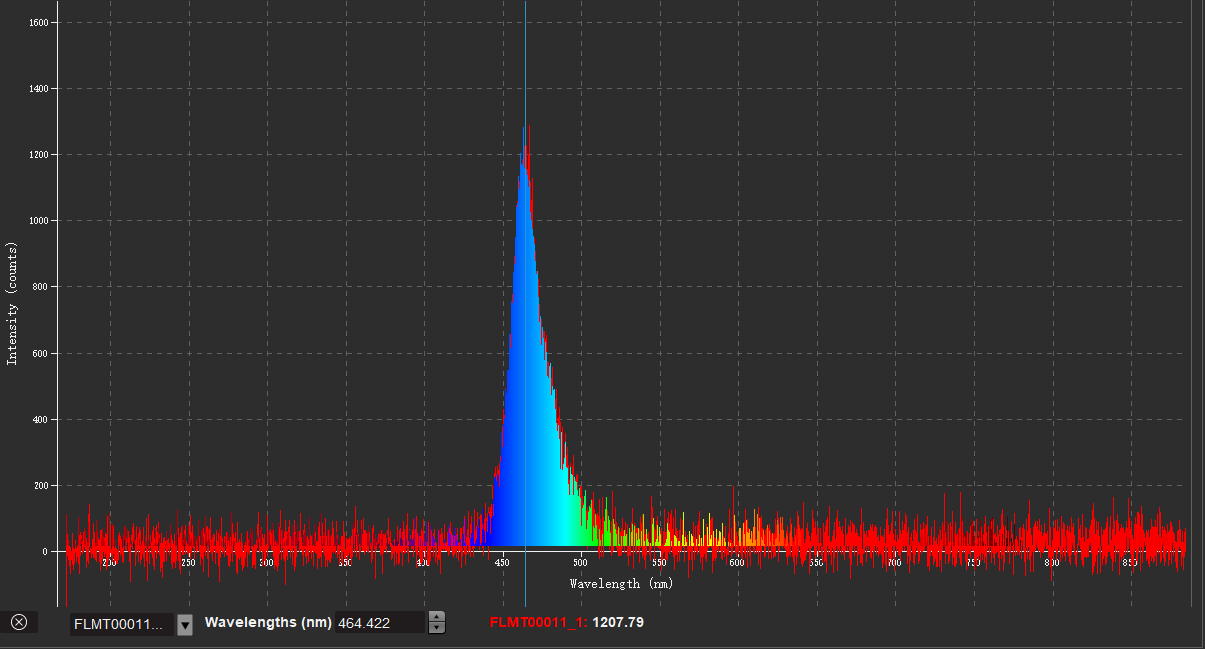
\includegraphics[width=\textwidth]{figures/blue_led.PNG}
    \caption{Blue LED}
  \end{subfigure}
  \caption{Spectographs for the LEDs}
\end{figure}

\begin{table} [H]
  \centering
  \begin{tabular}{|l|l|l|l|l|}
    \hline
    LED color	 & 	Voltage (V)	 & 	Wavelength (nm)	 & 	Frequency (Hz)	 & 	Energy (J) \\ \hline
    Red	 & 	1.7101	 & 	654.4	 & 	$ 4.58 \times 10 ^{14} $	 & 	$ 4.429 \times 10^{-19} $ \\ \hline
    Orange	 & 	1.8853	 & 	609.289	 & 	$ 4.92 \times 10 ^{14} $	 & 	$ 3.016 \times 10^{-19} $ \\ \hline
    Yellow-orange	 & 	1.891	 & 	589.533	 & 	$ 5.089 \times 10 ^{14} $	 & 	$ 3.026 \times 10^{-19} $ \\ \hline
    Blue	 & 	2.7608	 & 	464.422	 & 	$ 6.46 \times 10 ^{14} $	 & 	$ 2.736 \times 10^{-19} $ \\ \hline
  \end{tabular}

    \caption{Table of Voltages and Wavelengths to Calculate Planck's Constant}
  \label{table1}

\end{table}

To get frequency we use $ f = \frac{c}{\lambda } $ and to get energy we use the conversion $ E = \frac{V}{e} $ where $ e = 1.602 \times 10^{-19}  $ since volts are in units of Joules/Coulomb

%--- Analysis ---
\section{Analysis}

\subsection{Investigation 1}

The gas discharge tube produces light at very specific frequencies as displayed in \figurename \ref{gas1spec}.
A gas discharge tube is made up of a gas-containing tube with an electrode at either end.
When an electric potential is applied to the tube, the atoms in the gas molecules ionize, allowing charge to flow through the tube.
Because of the energy input from the electrodes, the electrons of the atoms gain kinetic energy, causing the electrons to jump to a higher energy orbital.
Then, when the electron jumps back down to a lower energy orbital, it releases a photon of a specific wavelength depending on these energy levels.
The distinct wavelengths can be observed in the spectrograph as spikes.

In this investigation, we also observed the non-spiky -- flat -- regions of the spectrograph.
Since these photons do not lie on an obvious wavelength peak, we assume that they are simply random noise from other, less prominent, light sources.
The central limit theorem says that the sampling distribution of the mean will be normally distributed, as long as the sample size is large enough.
Thus we used the histogram tool in excel over a 50 nm flat region, and observed that the intensity followed a Gaussian distribution (\figurename \ref{histo}.
The theoretical Gaussian distribution, using values of $ \sigma = 39.221$ and $ \mu = 13.916 $ which were found using the data, is shown in \figurename \ref{gauss}.

\begin{figure} [H]
  \center
  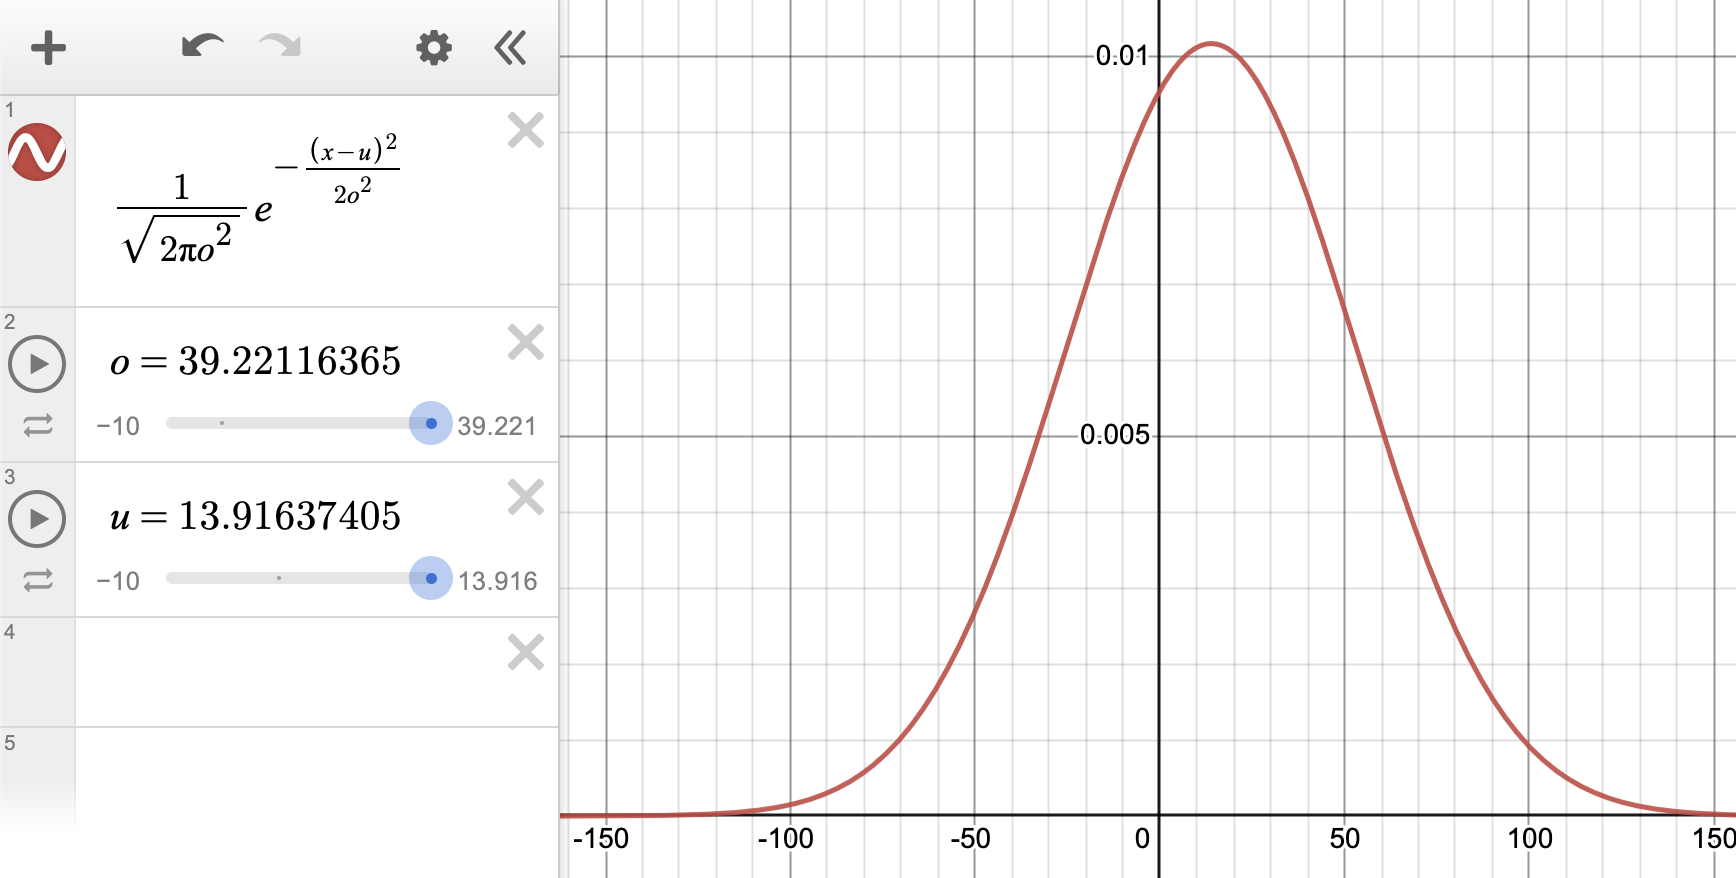
\includegraphics[width=0.65\textwidth]{figures/gaussian.png}
  \caption{Gaussian Distribution with $ \sigma = 39.221$ and $ \mu = 13.916 $}
  \label{gauss}
\end{figure}

Thus we see that the random noise follows a Gaussian Curve.

\subsection{Investigation 2}

In \figurename \ref{gas2} we see the spectrograph of the second gas discharge tube.
The spectrum matches that of the atomic spectrum for helium, seen below in \figurename \ref{helum_spectrum}.
The light emitted by the gas is the result of helium electrons moving from the outer, higher energy, orbits to lower orbits, releasing a photon of a specific wavelength depending on the initial and final orbit states.
The spikes in the spectrograph correspond to the wavelength of photons emitted by the electron movement.
We would predict that the spikes should be infinitely narrow because they depend on discrete wavelengths, however there is some width in the measured spectrograph.
Part of this result could be explained by equipment inaccuracy, and also the error could be explained by the Doppler effect.
The photons aren't the only particles moving in the tube -- the atoms themselves also move at an extremely excited state with high kinetic energy.
Thus, the wavelength of the emitted photons will be red-shifted when the atoms move away from the sensor, and blue-shifted when moving towards the sensor.
We estimate that 70 \% of the energy output is in the visible spectrum, which is less efficient than the other light sources we observed.

\begin{figure} [H]
  \center
  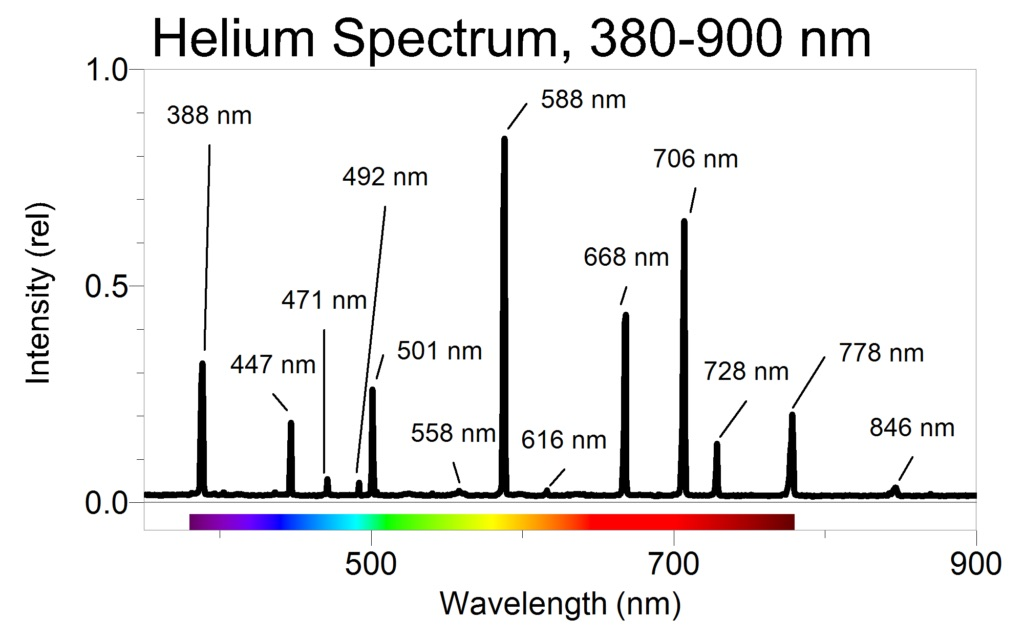
\includegraphics[width=0.65\textwidth]{figures/helium_spectra.jpeg}
  \caption{Helium Atomic Spectrum ({\tiny https://www.vernier.com/vernier-ideas/a-quantitative-investigation-of-the-helium-spectrum} )}
  \label{helum_spectrum}
\end{figure}

Fluorescent bulbs emit photons when electrons enter higher energy levels after bumping into other subatomic particles inside of the plasma within the bulb, thus operating similar to a gas discharge tube.
The difference is with the fluorescent tube's phosphor coating. 
Phosphors are substances that emit photons when they are exposed to light, photons with less energy than the ones absorbed since some energy is lost as heat.
This behavior produces the similar white light.
Almost all of the photons emitted by the bulb are within the visible spectrum, so the efficiency is quite good.
We estimate that 95 \% of the photons are within the visible spectrum (see \figurename \ref{flour}).

An incandescent bulb emits photons by running an electric current through a (tungsten) wire.
The light bulb filament gets to about 3000 K, so it gives off blackbody radiation, losing a lot of the energy to heat.
Since the temperature is so high, the peak EM emission is in the visible spectrum. 
Spectral radiance is given by Planck's law: $ B_{\lambda}(\lambda,T) = \frac{2hc^2}{\lambda ^{5} } \frac{1}{e^{hc / (\lambda k_{b}T)-1} } $.
We estimate that the fraction of energy output in the visible wavelengths is 85 \%.
Compared to the fluorescent bulb, this is not as efficient.

A halogen bulb is very similar to an incandescent bulb, but is just filled with halogen gas.
They also have tungsten filaments, but the particles burning off of the filament are redeposited back onto the filament by the halogen gas, allowing for the particles to be reused.
Halogen bulbs also operate at higher temperatures, increasing the frequency of its EM emissions.
In terms of efficiency, the halogen bulb is similar to the incandescent bulb in that it emits close to 85 \% of its light in the visible spectrum (\figurename \ref{bbrad})

The red and green lasers work by energizing atoms in a way to emit a certain wavelength of photon. We see in \figurename \ref{lasers} that this results in a very narrow wavelength spectrum centered on a specific wavelength.

\subsection{Investigation 3}

LED stands for Light Emitting Diode.
LED lamps emit light through a phenomenon called electroluminescence.
This phenomenon classifies when electrons fall into empty holes from the P-type semiconductor or when electrons collide with other electrons, exciting the struck electron.
Different materials in the LED produce different colors when voltages are applied across the diode, and the colors are generally monochromatic.
For each LED, we converted the peak wavelengths to frequencies, and the voltages to energy as seen in Table \ref{table1}.
We then used the relationship given in \eqref{ehf} to find Planck's constant knowing that $ h=\frac{E}{f} $.
\figurename \ref{linear_approx} show the method to approximate Planck's constant from the data.
From the previous equation, we know the slope of the linear approximation must yield Planck's constant, since energy is on the y-axis and frequency is on the x-axis.
Thus we estimated Planck's constant to be $ h = 6.33 \times ^{-34}  $.

\begin{figure} [H]
  \center
  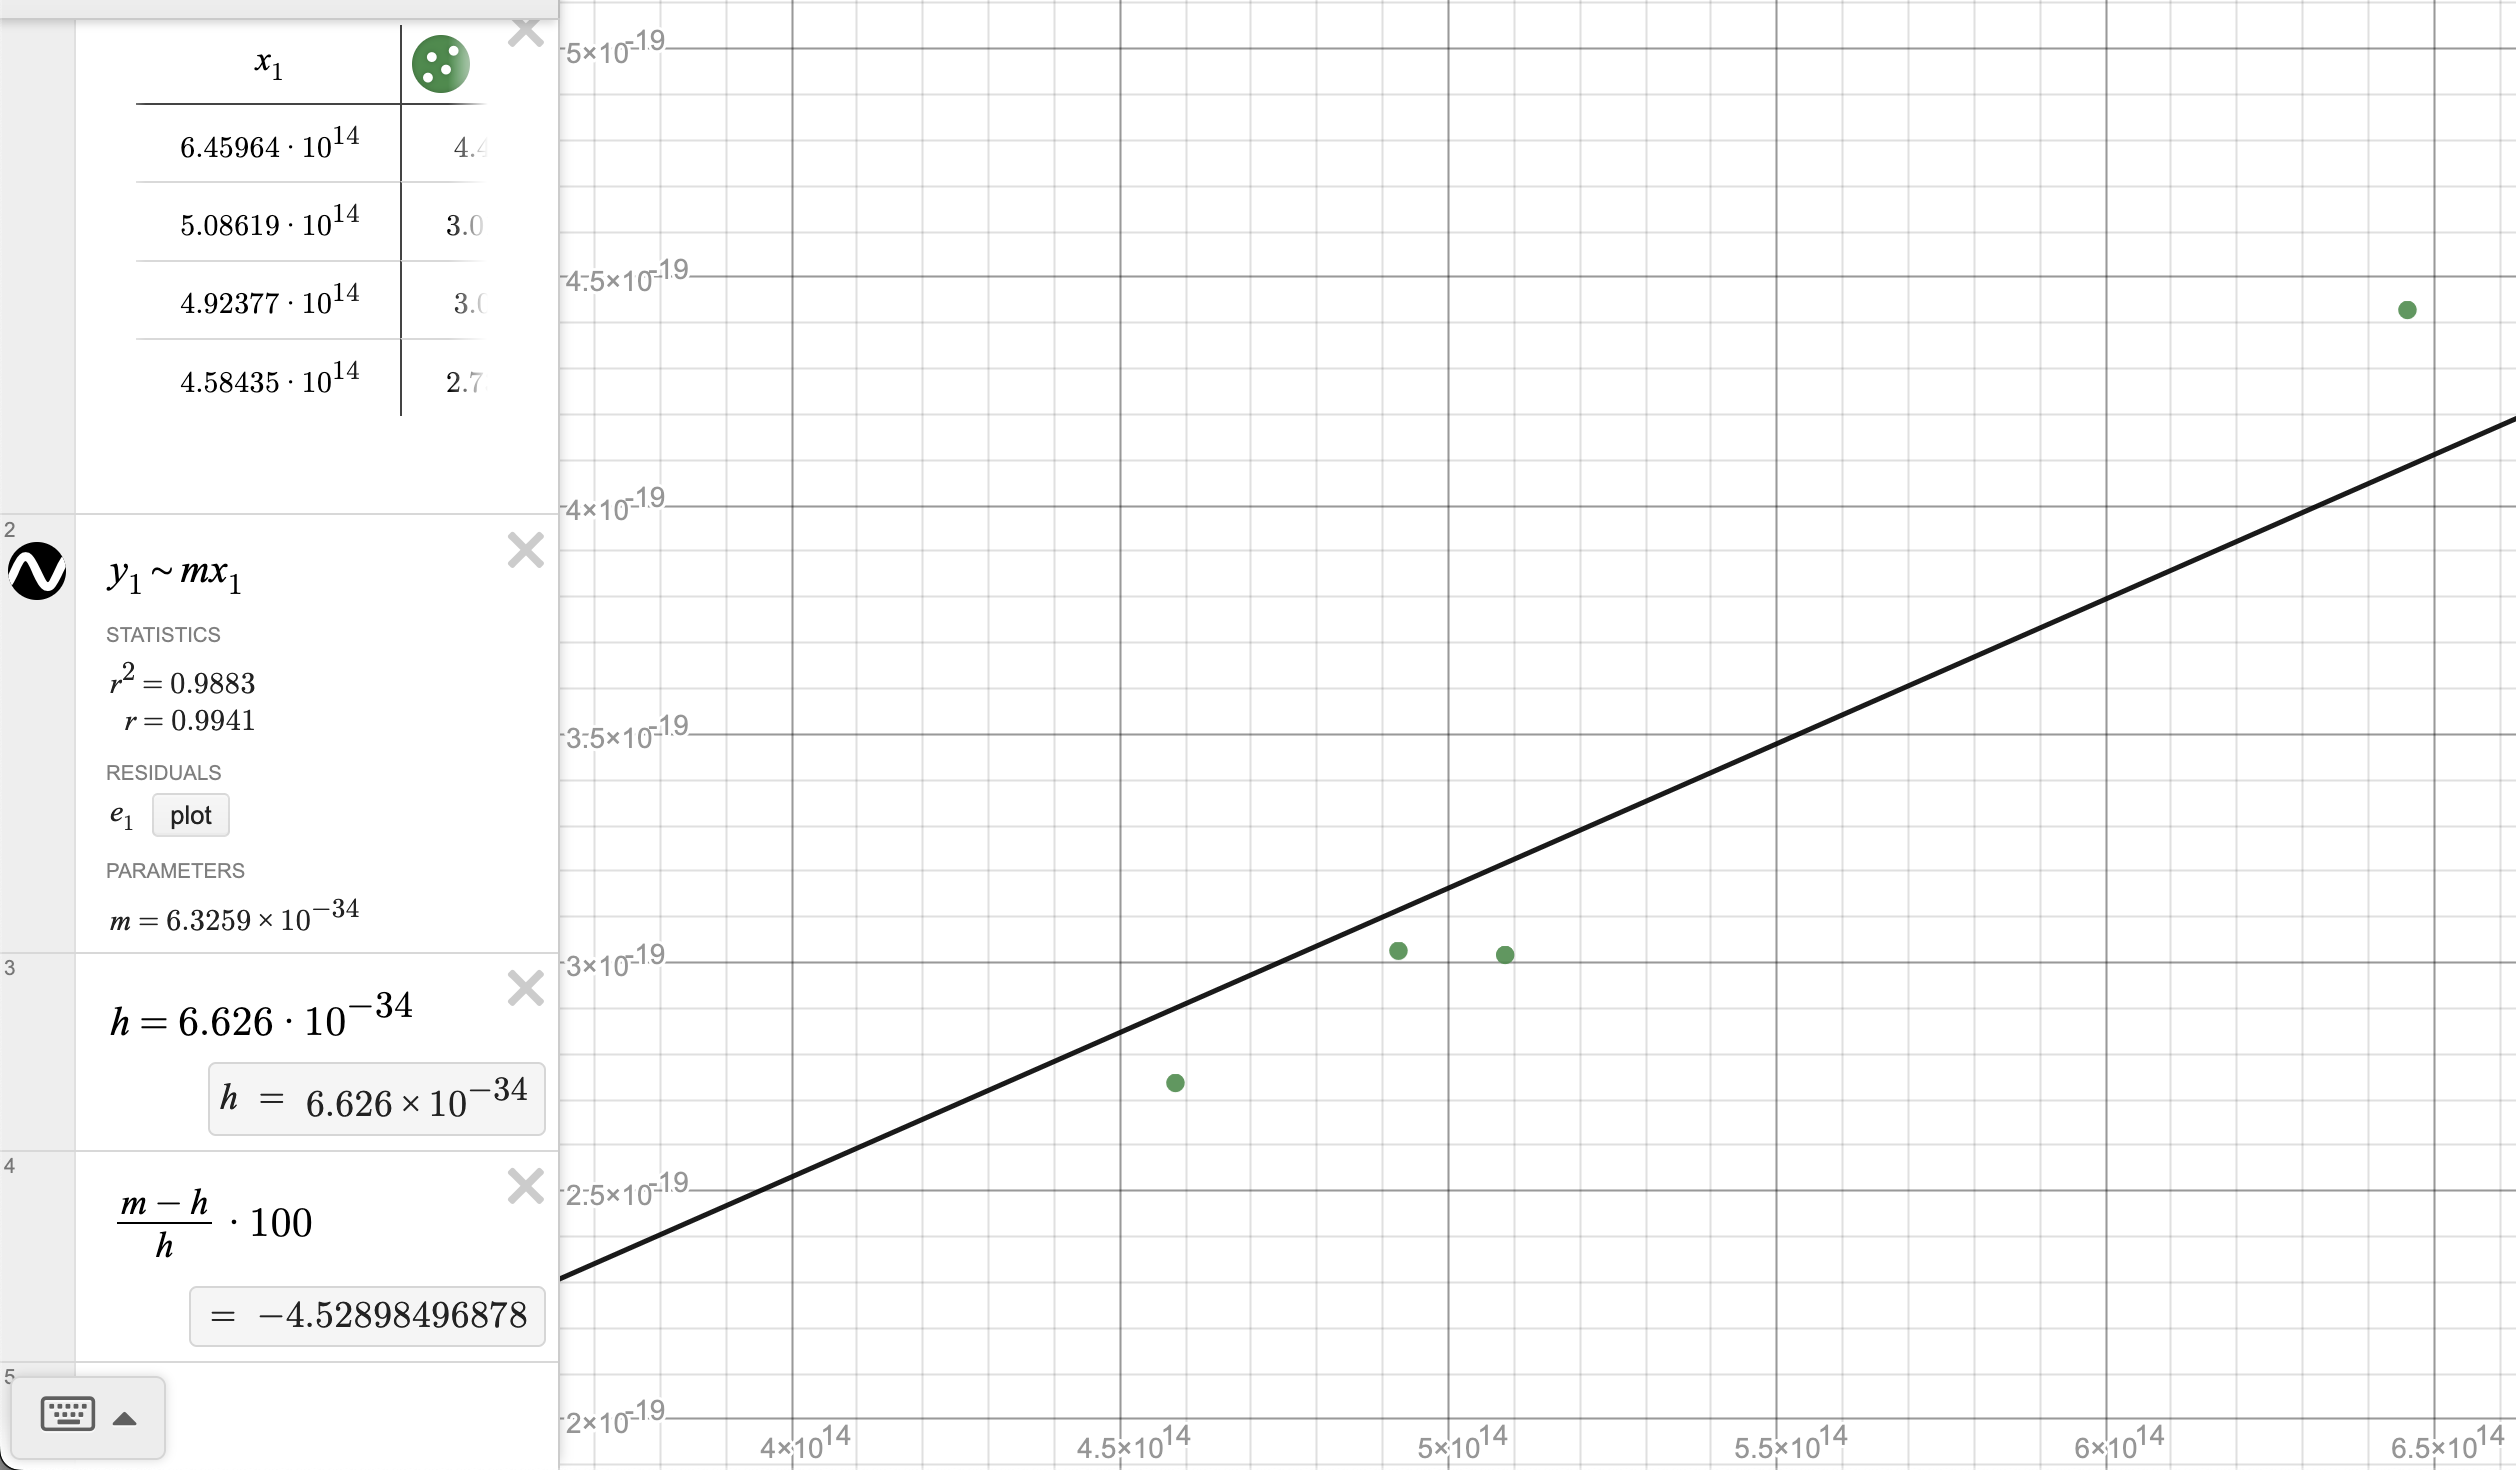
\includegraphics[width=0.75\textwidth]{figures/lin_approx.png}
  \caption{Finding Planck's Constant Using Table \ref{table1}}
  \label{linear_approx}
\end{figure}

%--- Results ---
\section{Results}

In Investigation 1, we observed that the histogram of the random background noise matches that of a Gaussian distribution.
In Investigation 2, we discovered that the incandescent and halogen bulbs display light spectra like other blackbody radiators. The gas discharge tubes and fluorescent bulb, however, have distinct peaks at certain wavelengths, indicating that the emissions are due to electrons relaxing from higher energy orbitals.
Finally, in Investigation 3, we calculated Planck's constant of $ h=6.33 \times 10 ^{-34}  $, which is a $ 4.53 \% $ error from the actual value.

\noindent \textbf{Sources of Error:}

For Investigation 2, we had to line up the optical fiber with the light manually. The fiber may have been slightly askew relative to the light source, altering the data in the graph. 
We noticed that when we swept the fiber across a light source, the graphs would behave slightly differently.
Furthermore, the calibration of the spectrometer may have been slightly off. This error would lead to a graph showing the EM radiation slightly skewed towards either UV or IR. This error could effect our perceptions of the energy efficiency of the bulbs.

For investigation 3, the largest source of error is probably involving the measured wavelength of the LED's emissions.
When reporting the wavelength of the light emitted from the LED, we tried to pick a wavelength in the middle of the peak, but at times this choice seemed arbitrary. We estimate that we were off by around 10 nm for each LED which would lead to some error in the regression.

%--- Conclusion ---
\section{Conclusion}

In this lab we were able to accomplish our primary objectives: show how background optical noise matches a Gaussian distribution, observing blackbody radiation vs discrete atomic spectra, and measuring Planck's constant from different LEDs to a commendable accuracy.

\end{document}
